\documentclass[12pt]{article}
\usepackage{graphicx}

\begin{document}

\begin{center}
	{\bf Teorema della Circuitazione di Ampere}
\end{center}

Il Teorema della Circuitazione di Ampere pu\'o esser scritto nel seguente modo:
\begin{equation}
	C_{\gamma}(\vec{B}) = \mu_0 i
\end{equation}
Oppure, pu\'o esser scritto cos\'i
\begin{eqnarray}
	\int_{\gamma}\vec{B}\cdot\vec{l} = \mu_0 i
\end{eqnarray}

\begin{figure}[h]
	\begin{center}
		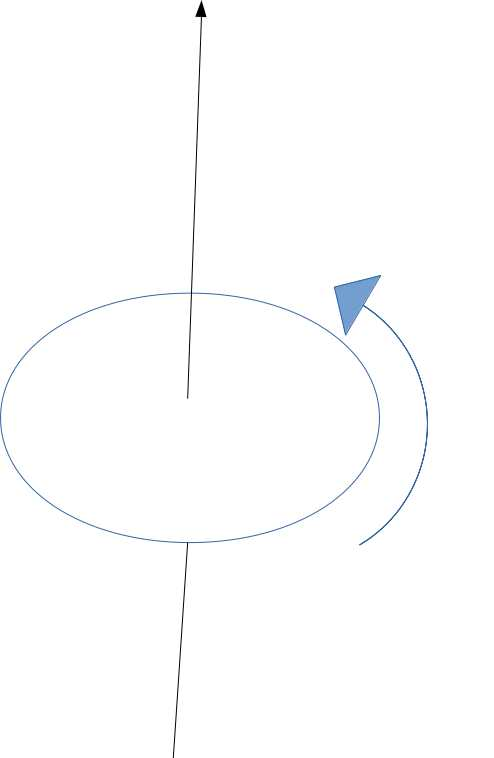
\includegraphics[width=4cm]{campoB.jpg}
		\caption{Circuito circolare visto in prospettiva ove viene effettuata la circuitazione del campo di induzione magnetica $\vec{B}$}
	\end{center}
\end{figure}

\section{Introduction}

Calcolare esercizio pag 376 n 282

\begin{itemize}
	\item $\left(x^2-3\right)\left(x^2+3\right)\left(x^4+9\right) =$ \\
	\item $= \left(x^4-9\right)\left(x^4+9\right) = $
	\item $= \left(x^8-81\right) $
\end{itemize}

\end{document}